\let\negmedspace\undefined
\let\negthickspace\undefined
\documentclass[journal]{IEEEtran}
\usepackage[a5paper, margin=10mm, onecolumn]{geometry}
\usepackage{lmodern} % Ensure lmodern is loaded for pdflatex
\usepackage{tfrupee} % Include tfrupee package

\setlength{\headheight}{1cm} % Set the height of the header box
\setlength{\headsep}{0mm}     % Set the distance between the header box and the top of the text

\usepackage{gvv-book}
\usepackage{gvv}
\usepackage{cite}
\usepackage{amsmath,amssymb,amsfonts,amsthm}
\usepackage{algorithmic}
\usepackage{graphicx}
\usepackage{textcomp}
\usepackage{xcolor}
\usepackage{txfonts}
\usepackage{listings}
\usepackage{enumitem}
\usepackage{mathtools}
\usepackage{gensymb}
\usepackage{comment}
\usepackage[breaklinks=true]{hyperref}
\usepackage{tkz-euclide} 
\usepackage{listings}
\def\inputGnumericTable{}                                 
\usepackage[latin1]{inputenc}                                
\usepackage{color}                                            
\usepackage{array}                                            
\usepackage{longtable}                                       
\usepackage{calc}                                             
\usepackage{multirow}                                         
\usepackage{hhline}                                           
\usepackage{ifthen}                                           
\usepackage{lscape}

\begin{document}

\bibliographystyle{IEEEtran}
\vspace{3cm}

\title{10.3.3.3.5}
\author{EE24BTECH11036 - Krishna Patil}
% \maketitle
% \newpage
% \bigskip
{\let\newpage\relax\maketitle}

\renewcommand{\thefigure}{\theenumi}
\renewcommand{\thetable}{\theenumi}
\setlength{\intextsep}{10pt} % Space between text and floats

\renewcommand{\thefigure}{\theenumi}
\renewcommand{\thetable}{\theenumi}
\setlength{\intextsep}{10pt} % Space between text and floats


\textbf{Question} : A fraction becomes $\frac{9}{11}$, if $2$ Is added to both the numerator and the denominator. If, $3$ is added to both numerator and denominator it becomes $\frac{5}{6}$. Find the fraction . \\

\solution
Let the fraction be $\frac{x}{y}$ then, according to the statements in the question ,
\begin{align}
\frac{x+2}{y+2} &= \frac{9}{11} \\
11x + 22 &= 9y + 18 \\
11x - 9y &= -4 
\end{align}
and
\begin{align}
	\frac{x+3}{y+3} &= \frac{5}{6} \\
	6x+18 &= 5y+15 \\
	6x - 5y &= -3
\end{align}
\textbf{CODING LOGIC}\\


	Let us assume the given system of equations are consistent and we will try solving using LU decomposition
	
	Given the system of linear equations:
	\begin{align}
		11x-9y &= -4 \\
		6x-5y &= -3
	\end{align}
	
	We rewrite the equations as:
	\begin{align}
		x_1 &= x, \\
		x_2 &= y,
	\end{align}
	giving the system:
	\begin{align}
		11x_1 - 9x_2 &= -4, \\
		6x_1 - 5x_2 &= -3.
	\end{align}
	
	\subsection*{Step 1: Convert to Matrix Form}
	We write the system as:
	\begin{align}
		A \mathbf{x} &= \mathbf{b},
	\end{align}
	where:
	\begin{align}
		A &= \begin{bmatrix} 11 & -9 \\ 6 & -5 \end{bmatrix}, \\
		\mathbf{x} &= \begin{bmatrix} x_1 \\ x_2 \end{bmatrix}, \\
		\mathbf{b} &= \begin{bmatrix} -4 \\ -3 \end{bmatrix}.
	\end{align}
	
	\subsection*{Step 2: LU factorization using update equaitons}
    Given a matrix $ \mathbf{A} $ of size $ n \times n $, LU decomposition is performed row by row and column by column. The update equations are as follows:\\
    \textbf{Step-by-Step Procedure:}\\
1. Initialization: 
   - Start by initializing $ \mathbf{L} $ as the identity matrix $ \mathbf{L} = \mathbf{I} $ and $ \mathbf{U} $ as a copy of $ \mathbf{A} $.
   
2. Iterative Update:
   - For each pivot $ k = 1, 2, \ldots, n $:
     - Compute the entries of $ U $ using the first update equation.
     - Compute the entries of $ L $ using the second update equation.
   
3. Result:
   - After completing the iterations, the matrix $ \mathbf{A} $ is decomposed into $ \mathbf{L} \cdot \mathbf{U} $, where $ \mathbf{L} $ is a lower triangular matrix with ones on the diagonal, and $ \mathbf{U} $ is an upper triangular matrix.

    

\subsection*{1. Update for $ U_{k,j} $ (Entries of $ U $)}

For each column $ j \geq k $, the entries of $ U $ in the $ k $-th row are updated as:
\[
U_{k,j} = A_{k,j} - \sum_{m=1}^{k-1} L_{k,m} \cdot U_{m,j}, \quad \text{for } j \geq k.
\]
This equation computes the elements of the upper triangular matrix $ \mathbf{U} $ by eliminating the lower triangular portion of the matrix.

\subsection*{2. Update for $ L_{i,k} $ (Entries of $ L $)}

For each row $ i > k $, the entries of $ L $ in the $ k $-th column are updated as:
\[
L_{i,k} = \frac{1}{U_{k,k}} \left( A_{i,k} - \sum_{m=1}^{k-1} L_{i,m} \cdot U_{m,k} \right), \quad \text{for } i > k.
\]
This equation computes the elements of the lower triangular matrix $ \mathbf{L} $, where each entry in the column is determined by the values in the rows above it.\\
Using a code we get L,U as 
\begin{align}
	L&=\begin{bmatrix} 1.00 & 0.00 \\ \frac{6}{11} & 1.00 \end{bmatrix}         \\
		U&=\begin{bmatrix} 11.00 & -9.00 \\ 0.00 & -\frac{1}{11} \end{bmatrix}
\end{align}
So, solving the $A\textbf{x}= \textbf{b}$ we get, $x=7$ and $y=9$, the fraction is $\frac{7}{9}$.

\begin{figure}[h!]
    \centering
    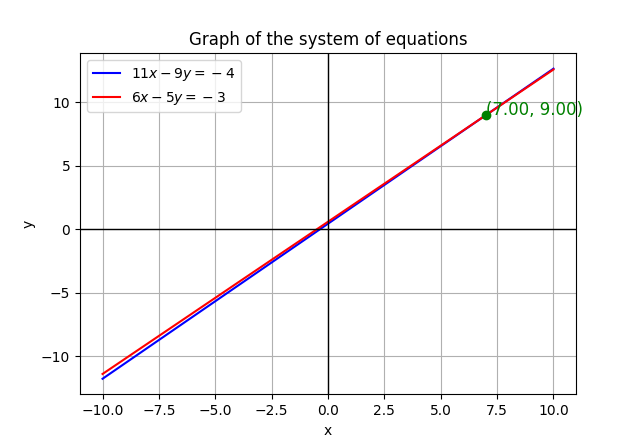
\includegraphics[width=0.7\columnwidth]{fig/Figure_1.png}
    \label{label}
\end{figure}	
\end{document}
